\documentclass{beamer}
\usepackage{../tut-slides}
\usepackage{../mathoperatorsAuD}

\usepackage{amsmath,amssymb}
\usepackage{enumerate}
%\usepackage[inline]{enumitem} 		%customize label
%\newcommand{\labelitemi}{\raisebox{1pt}{\scalebox{.9}{$\blacktriangleright$}}}
%\newcommand{\labelitemii}{$\vartriangleright$}
%\newcommand{\labelitemiii}{--}
\setbeamertemplate{itemize item}{\raisebox{1pt}{\scalebox{.9}{$\blacktriangleright$}}}
\setbeamertemplate{itemize subitem}{$\vartriangleright$}

\usepackage{booktabs}
\usepackage{tabularx}
\usepackage{tabu}
\newcommand*\head{\rowfont{\bfseries}}
\newcommand*{\tw}{\rowfont{\ttfamily}}
\renewcommand{\tabularxcolumn}[1]{>{\hspace{0pt}}m{#1}}

\usepackage{cancel}

%%%% EBNF-Terme %%%%
\newcommand{\wdh}[1]{\hat{\{} \ #1 \ \hat{\}}}
\newcommand{\opt}[2]{\hat{(} \ #1 \ \hat{|} \ #2 \ \hat{)}}
\newcommand{\byp}[1]{\hat{[} \ #1 \ \hat{]}}
\newcommand{\rdb}[1]{\hat{(} \ #1 \ \hat{)}}

\begin{document}	
	\title{Algorithmen und Datenstrukturen}
	\subtitle{Übung 2: Syntaxdiagramme \& EBNF}
	\author{Eric Kunze}
	\email{eric.kunze@mailbox.tu-dresden.de}
	\city{TU Dresden}
%	\institute{Lehrstuhl für Grundlagen der Programmierung}
	\titlegraphic{
\includegraphics[width=2cm]{../TUD-white.pdf}}
	\date{06.11.2020}

	\maketitle


%%%%%%%%%%%%%%%%%%%%%%%%%%%%%%%%%%%%%%%%%%%%%%%%%%%%%%%%%%%%%%%%%%%%%%%%%%%%%

\begin{frame} \frametitle{Videoempfehlungen}
	
	\textbf{Prof. Dr. Markus Krötzsch:}
	\begin{itemize}
		\item  \url{https://youtu.be/Lma6jaPnD-I}
	\end{itemize}	
	
	\pause\bigskip
		
	\textbf{Tutorials für \texttt{C}:}
	\begin{itemize}
		\item freeCodeCamp.org \\
		\url{https://www.youtube.com/watch?v=KJgsSFOSQv0&ab_channel=freeCodeCamp.org}
		\item SEPL Goethe University Frankfurt \\
		\url{https://www.youtube.com/watch?v=CeEfTlRFEA0&t=113s&ab_channel=SEPLGoetheUniversityFrankfurt}
		\item Caleb Curry: \\
		\url{https://www.youtube.com/watch?v=Bz4MxDeEM6k&list=PL_c9BZzLwBRKKqOc9TJz1pP0ASrxLMtp2&ab_channel=CalebCurry}
	\end{itemize}
\end{frame}

\section{Syntaxdiagramme}

\begin{frame} \frametitle{Syntaxdiagramme \& Rücksprungalgorithmus}
	\small
	\begin{itemize}
		\item syntaktische Variable = Nichtterminalsymbol = Name eines Syntaxdiagramms
		\item Jedes Kästchen ist mit dem Namen eines Syntaxdiagramms beschriftet.
		\item Jedes Oval ist mit einem Terminalsymbol beschriftet.
	\end{itemize}

	\pause

	\textbf{Rücksprungalgorithmus}
	\begin{itemize}
		\item jedes Kästchen bekommt eindeutige Marke (Rücksprungadresse)
		\item beim Betreten eines Syntaxdiagramms wird eine Marke auf den Keller gelegt
		\item Nachweis von Zugehörigkeit eines Wortes zu einer Sprache
	\end{itemize}
\end{frame}

\begin{frame} \frametitle{Aufgabe 1}
	\begin{itemize}
		\item Teil (a) ---
		z.B. $\epsilon, a, c, caa, aaaa, \dots$
		\item Teil (b) ---
		z.B. $aaac, abacac, abbaccac, \dots$
		\item 	Teil (c) ---
		z.B. $\epsilon, ab, abab, ac, aabcab, \dots$
	\end{itemize}
\end{frame}

\begin{frame} \frametitle{Aufgabe 2 --- Teil (a)}
	\begin{minipage}{\dimexpr0.5\linewidth-\fboxrule-\fboxsep}
		\small
		\textbf{Protokollierungszeitpunkte:}
		\begin{itemize}
			\item jeder Aufenthalt in einem Syntaxdiagramm entspricht einer Zeile
			\item jede Zeile führt eine Operation auf dem Markenkeller aus
			\item $\cancel{3}$ = Rücksprung zu Marke $3$
		\end{itemize}
	\end{minipage}
	\pause
	\begin{minipage}{\dimexpr0.5\linewidth-\fboxrule-\fboxsep}
		\centering
		\begin{tabular}{l|r}
			\hline
			Wort & Markenkeller \\ \hline \pause
			a & 1 \\ \pause
			a & 31 \\ \pause
			aa & 131 \\ \pause
			aaa & 2131 \\ \pause
			aaa & 32131 \\ \pause
			aaaaccb & $\cancel{3} 2131$ \\ \pause
			aaaaccb & $\cancel{2}131$ \\ \pause
			aaaaccbd & $\cancel{1}31$ \\ \pause
			aaaaccbdb & $\cancel{3}1$ \\ \pause
			aaaaccbdb & $\cancel{1}$ \\ \pause
			aaaaccbdbb & -- \\ \hline
		\end{tabular}
	\end{minipage}
\end{frame}

\begin{frame} \frametitle{Aufgabe 2 --- Teil (b)}
	\begin{align*}
		L &= \menge{a^{2i} c b^{3i} c^k d^{2k+1} \mid i > 0, k \ge 0} \\
		&= \menge{a^{2i} c b^{3i} \mid i > 0} * \menge{c^k d^{2k+1} \mid k \ge 0}
	\end{align*}
	
	\centering
	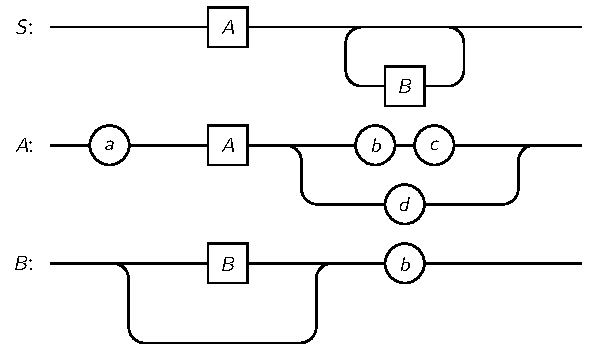
\includegraphics[width=.9\textwidth]{tut02_syntax-dia-2a.pdf}
\end{frame}


\section{Extended Backus-Naur-Form}

\begin{frame} \frametitle{EBNF-Definition}
	\small
	\begin{itemize}
		\item EBNF-Definition besteht aus endlicher Menge von EBNF-Regeln.
		\item Jede EBNF-Regel besteht aus einer linken und einer rechten Seite, die rechte Seite ist ein EBNF-Term.
	\end{itemize}
	\pause
	\begin{block}{Definition: EBNF-Term}
		Seien $V$ eine endliche Menge (syntaktische Variablen) und $\Sigma$ eine endliche Menge (Terminalsymbole) mit $V \cap \Sigma = \emptyset$. Die Menge der EBNF-Terme über $V$ und $\Sigma$ (notiere: $T(\Sigma, V)$), ist die \emph{kleinste} Menge $T \subseteq \brackets{V \cup \Sigma \cup \menge{\hat{\{}, \hat{\}}, \hat{[}, \hat{]}, \hat{(}, \hat{)}, \hat{|}}}$ mit $V \subseteq T$, $\Sigma \subseteq T$ und
		\begin{itemize}
			\item Wenn $\alpha \in T$, so auch $\rdb{\alpha} \in T$, $\wdh{\alpha} \in T$, $\byp{\alpha} \in T$.
			\item Wenn $\alpha_1, \alpha_2 \in T$, so auch $\opt{\alpha_1}{\alpha_2} \in T$, $\alpha_1 \alpha_2 \in T$
		\end{itemize}
	\end{block}
\end{frame}

\begin{frame} \frametitle{Aufgabe 3 --- Teil (a)}
	\small
	EBNF-Definition $\mathcal{E} = (V,\Sigma,S,R)$ mit $\Sigma = \menge{a,b,c,d}$,
	\begin{align*}
		V = \menge{S,A,B} 
		\quad \und \quad
		R = \Big\{ S &::= A \ \wdh{B} , \\ 
				   A &::= aA \  \opt{bc}{d} , \\
				   B &::= \byp{B} \ b 
		    \Big\}
	\end{align*}

	\pause
	
	\textbf{Übersetzung in Syntaxdiagrammsystem:}
	
	\centering
	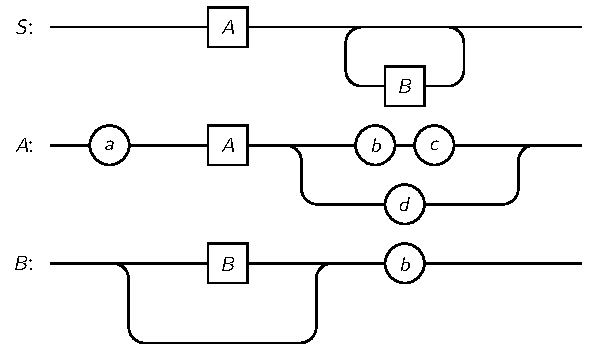
\includegraphics[height=4.5cm]{tut02_syntax-dia-3a.pdf}
\end{frame}

\begin{frame} \frametitle{Aufgabe 3 --- Teil (b)}
	Gegeben sei die Sprache
	\begin{equation*}
		L = \menge{(ab)^n c^{m+1} d^k b^{n+m} : n,m \ge 0, k \ge 1}
	\end{equation*}
	Gesucht ist eine zugehörige EBNF-Definition. \pause
	\begin{equation*}
		L = \menge{\textcolor{cdorange}{(ab)^n} \textcolor{cdpurple}{c^{m+1}} d^k \textcolor{cdpurple}{b^m} \textcolor{cdorange}{b^n} : n,m \ge 0, k \ge 1}
	\end{equation*}
	\pause 
	
	\textbf{EBNF-Definition:} $\mathcal{E} = (V,\Sigma,S,R)$ mit $\Sigma = \menge{a,b,c,d}$, 
	\begin{align*}
		V = \menge{S,A} \quad \und \quad
		R = \Big\{ 
			S &::= \opt{abSb}{A}, \\
			A &::= \opt{cAb}{cd \ \wdh{d}} \enskip 
		\Big\}
	\end{align*}
\end{frame}

\end{document}